\section{Designing the graphical layout}
\subsection{Drawing the scene}
Several considerations were made in regard to the graphical style for the program. The drawings should be easy to distinguish, funny-looking and relate to the theme of Christmas. 

The first step was to draw a suitable background that ultimately would create a Christmas mood. The original idea was to have a few different sets to choose from, depending on the time of the day or week. Due to time constrains only one background was drawn in the end. As shown on figure \ref{fig:ip_Background}, it consists of some mountain hills and a blue sky. It was important not to have too many details, since the focus should be on the characters themselves.

\begin{figure}[htbp]
\centering
\includegraphics[width=0.50\textwidth]{Pictures/Design/Background.png}
\caption{The background image used for the program.}
\label{fig:ip_Background}
\end{figure}

In addition, due to light conditions at the library, the colors chosen for the background are bright(see figure \ref{fig:background_projector}). This action was taken in order for the projector to output a usable illustration. If the colors were too dark, they would be difficult to see on the canvas.

To make the scene feel more alive, Christmas trees were added, as well as falling snowflakes.

\begin{figure}[htbp]
\centering
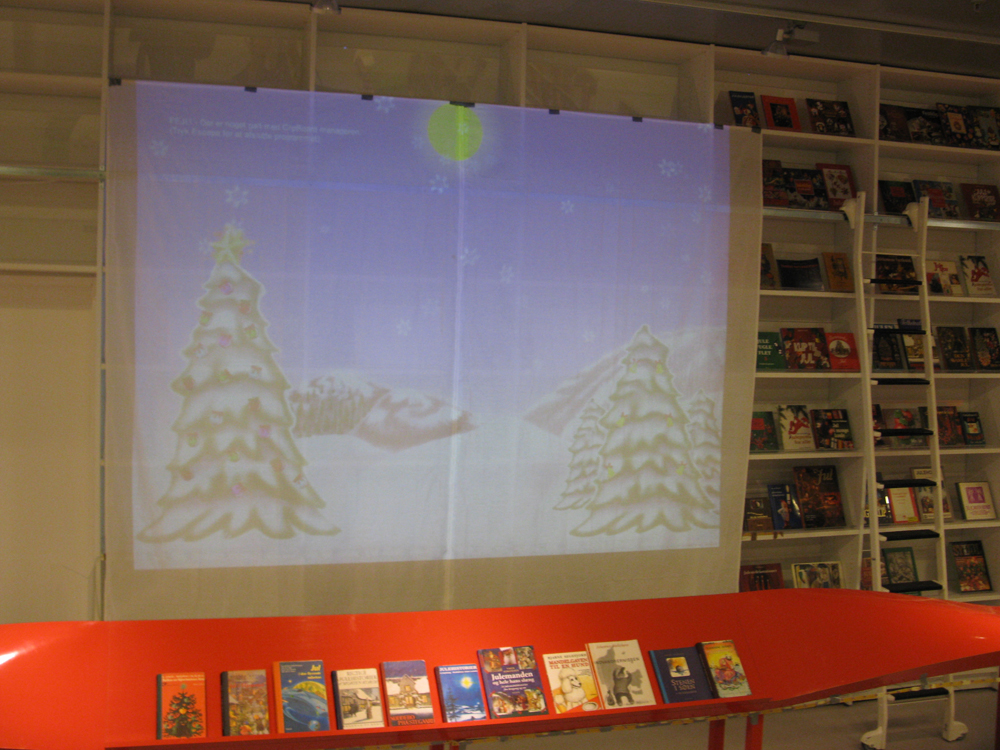
\includegraphics[width=0.50\textwidth]{Pictures/Design/background_projector}
\caption{The colors should be bright enough so they are clear on the canvas.}
\label{fig:background_projector}
\end{figure}

\subsection{Drawing the characters}
In addition to the background, a group of Christmas characters were made. It was decided to have a small selection of characters that were visually very different from each other: a snowman, a pixie boy, a pixie girl, an angle, and a squirrel.

It was decided to draw the characters by hand instead of using some pre-made drawings from the Internet. In the beginning outlines of the characters were drawn on sheets of paper (see figure \ref{fig:boy_sketch}). When the outlines was satisfying, they were imported to the computer and re-drawn in Photoshop using drawing tablets. The drawing tablets have pressure sensors, which make the line's thickness change according to pressure of the pen. Having different strokes makes the characters spring more to life. The last stage was then to color the characters, keeping a contrast to the background.

\begin{figure}[htbp]
\centering
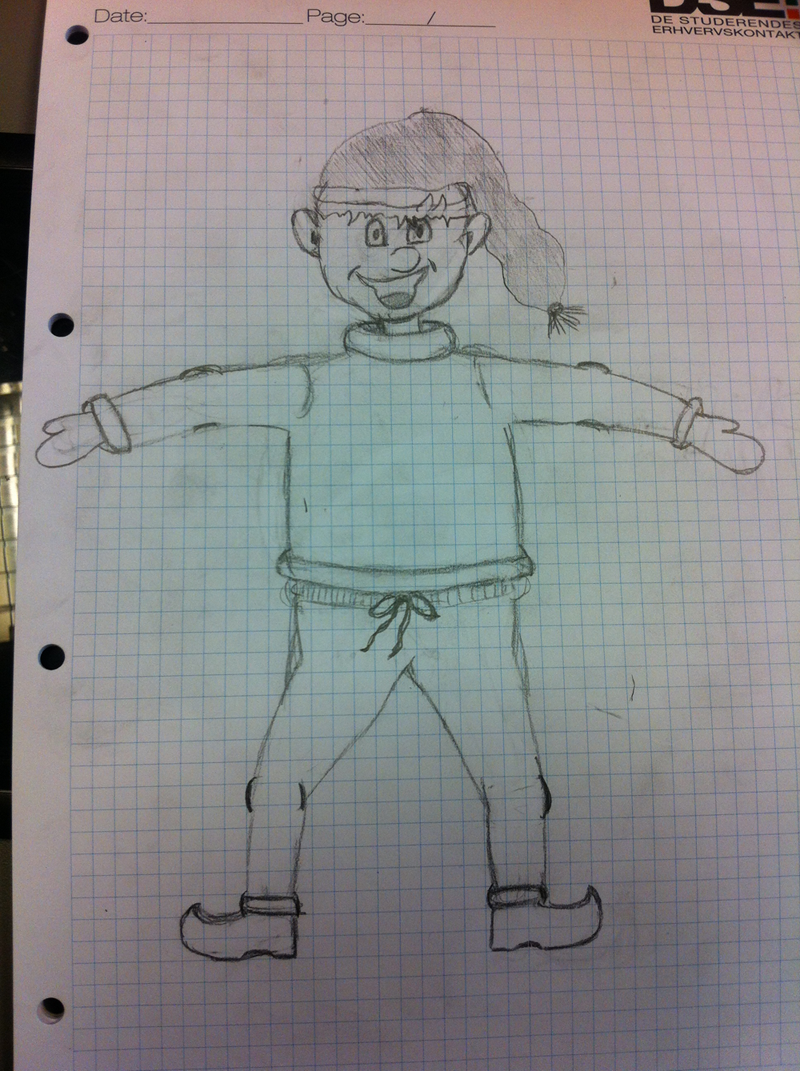
\includegraphics[width=0.50\textwidth]{Pictures/Design/boy_sketch}
\caption{The characters were first drawn on paper, then imported to and colored in Photoshop.}
\label{fig:boy_sketch}
\end{figure}

It was decided to give the characters a cartoon-like look. The style was chosen to appeal to a broader target group. This was done by using a variety of techniques. One of them was to create oversized body parts e.g. oversized heads. Two of the characters, the snowman and the angel is shown on figures \ref{fig:PixieGirl} and \ref{fig:Angel}.

\begin{figure}[htbp] \centering
\begin{minipage}[b]{0.45\textwidth} \centering

\includegraphics[width=1.00\textwidth]{Pictures/Design/snowman} % Venstre billede
\end{minipage} \hfill
\begin{minipage}[b]{0.45\textwidth} \centering
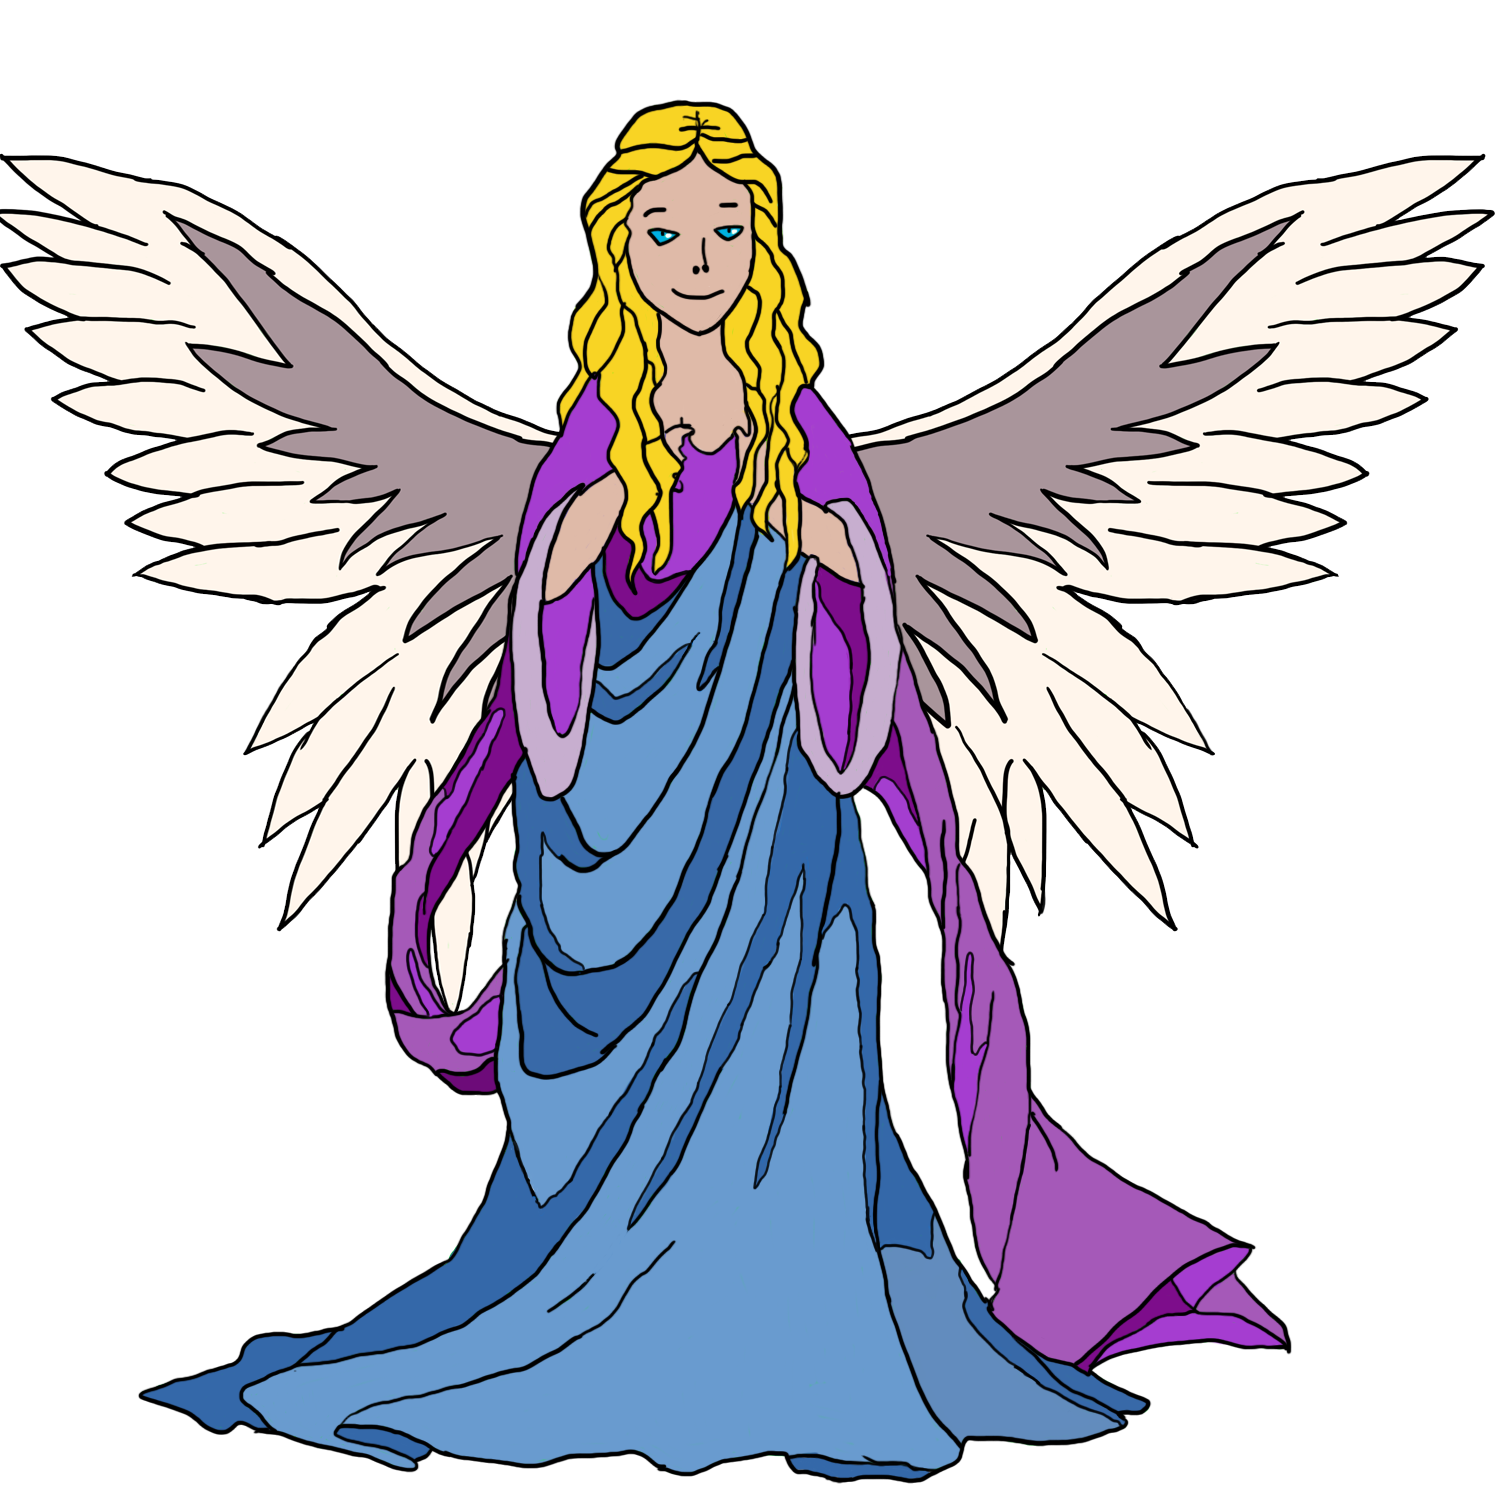
\includegraphics[width=1.00\textwidth]{Pictures/Design/Angel} % Højre billede
\end{minipage} \\ % Captions og labels
\begin{minipage}[t]{0.45\textwidth}
\caption{The snowman character.} % Venstre caption og label
\label{fig:PixieGirl}
\end{minipage} \hfill
\begin{minipage}[t]{0.45\textwidth}
\caption{The angle character.} % Højre caption og label
\label{fig:Angel}
\end{minipage}
\end{figure}

\subsection{Making animations}
In order to achieve more vivid characters, animations were added. It was decided to give the characters three animations for each movement. Even though they are quite simple, they create a sense of motion, making the characters appear more life-like. Each character has three sets of animation. The primary animation is an idle stance that will play whenever a visitor is standing still in front of the camera (see figure \ref{fig:squirrel_animation}). Then there are two walking animations: one for each direction (left and right).

\begin{figure}[htbp]
\centering
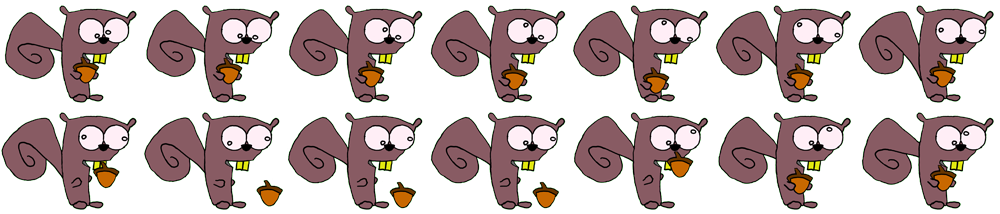
\includegraphics[width=1.00\textwidth]{Pictures/Design/squirrel_animation}
\caption{Idle animation for the squirrel.}
\label{fig:squirrel_animation}
\end{figure}

The animations were created as sprite sheets, which is a single image containing multiple frames. This approach was decided for practical purposes, since it is relatively easy to create a single character and then move small parts of it for each frame, such as arms, legs, and eyes. In the program the image is looped through, showing each frame for an amount of time. Figure \ref{fig:Design_PixieBoyWalking} shows an example of the pixie boy walk cycle that will play whenever a visitor is moving.

\begin{figure}[htbp]
\centering
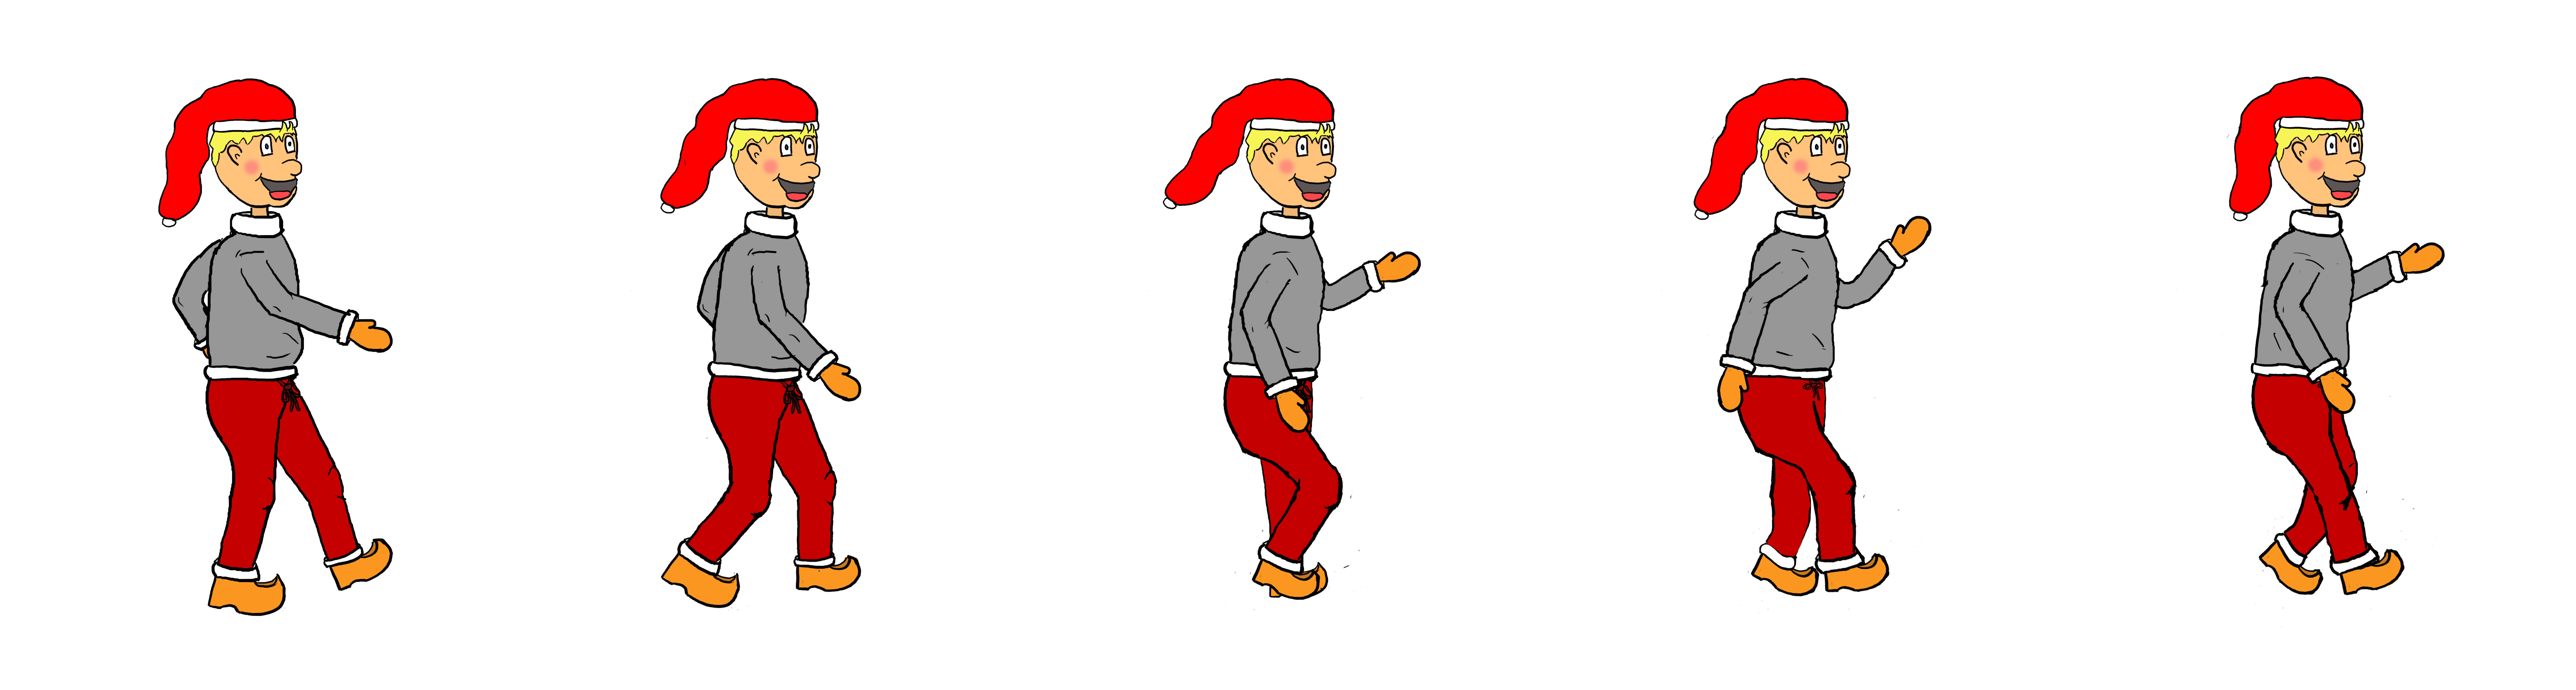
\includegraphics[width=1.00\textwidth]{Pictures/Design/PixieWalking.png}
\caption{The pixie boy walk cycle is looped through to create a sense of motion.}
\label{fig:Design_PixieBoyWalking}
\end{figure}